\subsection{Physics Engine}
\label{sub:Physics Engine}

\subsubsection{前言}

\paragraph{甚麼是遊戲物理引擎}

為了讓遊戲能夠更趨於真實,聰明的遊戲開發者就將物理學的知識與觀念融入到遊戲當中,試著用各種不同的物理參數來真實世界的情況。物理引擎又有兩種常見的類型,一種為實時的物理引擎和高精度的物理引擎。在遊戲物理中,會選擇使用實時的物理引擎,並在程式中想辦法降低演算法的複雜度,或許從中會犧牲少部分的精確度,但在不影響肉眼「看起來」的情況下是可以被接受的。而高精度的物理引擎,通常使用在科學研究(計算物理學)和電腦動畫電影製作上,對於細節比較講究的才會選擇使用高精度的物理引擎。

\subsubsection{常見的物理引擎介紹}

\paragraph{2D遊戲物理引擎}
\begin{itemize}
    \item{Box2D}
        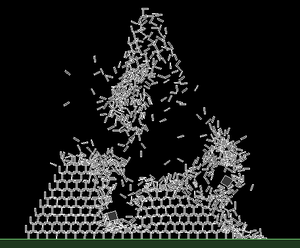
\includegraphics[height=0.2\linewidth]{./resources/physics/box2d(1).png} 
    \SubItem{一款免費的開源二維物理引擎,由Erin Catto使用C++編寫,在zlib授權下發布}
        \SubItem{著名遊戲}
            \SubSubItem{AngryBird}
                
\includegraphics[width=0.1\linewidth]{./resources/physics/angryBird.png}
        \SubItem{一個剛體動力學模擬引擎和一個碰撞檢測引擎,支援長方體、球體、圓柱體}
\end{itemize}

\paragraph{3D遊戲物理引擎}
\begin{itemize}
    \item{ODE}
        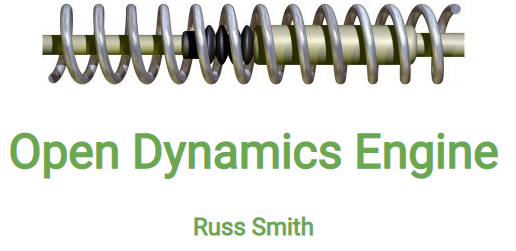
\includegraphics[height=0.2\linewidth]{./resources/physics/ODE(1).png}
        \SubItem{一個剛體動力學模擬引擎和一個碰撞檢測引擎,支援長方體、球體、圓柱體}
        \SubItem{著名遊戲}
            \SubSubItem{浩劫殺陣:車諾比之影}
                
\includegraphics[width=0.1\linewidth]{./resources/physics/ODE(2).png}
            \SubSubItem{X-Moto}
                 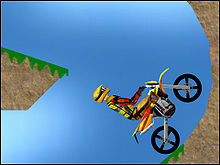
\includegraphics[width=0.1\linewidth]{./resources/physics/ODE(3).png}
    \item{Bullet}
        \includegraphics[height=0.2\linewidth]{./resources/physics/bullet(1).png}
        \SubItem{一個跨平台的開源物理引擎,支援三維碰撞檢測、柔體動力學和剛體動力學,多用於遊戲開發和電影製作中}
        \SubItem{著名遊戲}
            \SubSubItem{GTA 俠盜獵車手V}
                \includegraphics[width=0.1\linewidth]{./resources/physics/bullet(2).png} 
    \item{Havok}
        
\includegraphics[height=0.2\linewidth]{./resources/physics/havok(1).png}
        \SubItem{遊戲動力學開發工具包(Havok Game Dynamics SDK)}
        \SubItem{一個用於物理(動力學)效應模擬的遊戲引擎,為電子遊戲所設計,注重在遊戲中對於真實世界的模擬}
        \SubItem{著名遊戲}
            \SubSubItem{星海爭霸II:自由之翼}
                
\includegraphics[height=0.2\linewidth]{./resources/physics/havok(2).png}
            \SubSubItem{薩爾達傳說 - 曠野之息}
                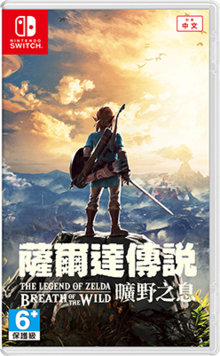
\includegraphics[height=0.2\linewidth]{./resources/physics/havok(3).png}
\end{itemize}

\note{以上內容出自維基百科}

\subsubsection{研究背景}

在大學期間,系上的相關撰寫遊戲課程當中,一般來說要運用物理模擬幾乎都會用到 Box2D 這個 2D 的物理引擎,但都往往無法深入探究裡面的實作以及其中的原理,頂多只會運用物理引擎的函式庫來時做遊戲。因此,想透過這次專題的機會,來深入探討 Box2D 其中的原理,試著自己實作看看簡單的物理模擬,將所學到的物理知識透過程式來實現出來,並將遊戲物理融合到這次的專案當中。

\subsubsection{研究歷程}
\begin{itemize}
    \item{拾回物理的理論}
    \item{搜尋網路資源}
        \SubItem{\href{https://github.com/erincatto/box2d-lite}{Box2d-lite}} 
        \SubItem{\href{https://code.google.com/archive/p/box2d/downloads}{Google Code Archive Box2d}}
        \SubItem{\href{https://github.com/phenomLi}{phenomLi}}
        \SubItem{\href{https://www.youtube.com/watch?v=SHinxAhv1ZE}{GDC2014 - Understanding Constraints}}
        \SubItem{\href{https://www.youtube.com/watch?v=NwPIoVW65p}{GDC2015 - Bend the Physics Engine to Your Will}}
        \SubItem{\href{http://allenchou.net/game-physics-series/}{AllenChou Game Physics series}}
    \item{閱讀相關技術文章,結果掉出同樣在研究遊戲物理來我個人網站上留言}
        \SubItem{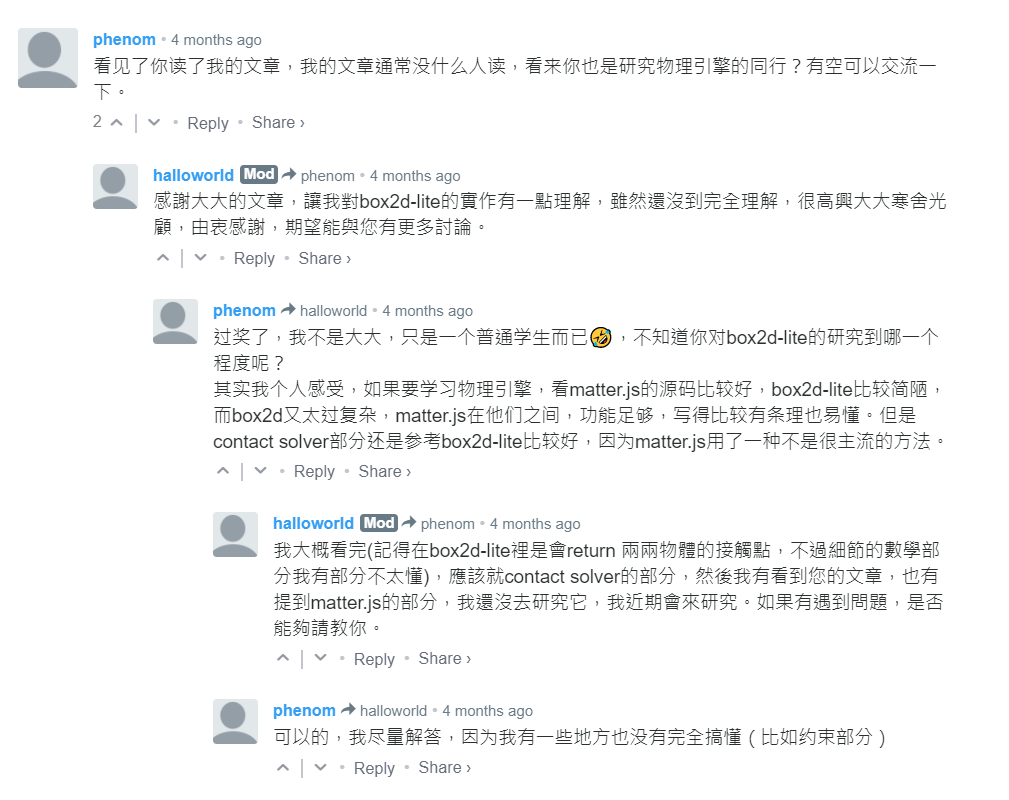
\includegraphics[width=\linewidth]{./resources/physics/comment.png}}
    \item{SITCON2020 - 你說這隻溫馴的繩嗎?}
        \SubItem{有資源可以詢問}
        \SubItem{藉此拿到遊戲物理界大老Allen Chou系列影片}
    \item{證明 Box2d 裡的一些物理公式,藉此驗證以及知其所以然}
    \item{融合進 RishEngine 當中}
    \item{參考其他開源專案的實作}
        \SubItem{Impulse Engine}
        \SubItem{了解圓、多邊形的 Contact Point 找法}
        \SubItem{藉此能夠實作 RishEngine 的圓、多邊形的碰撞}

    \subsubsection{懷疑與困難}
    \item{重造輪子的問題}
        \SubItem{在這個成熟的box2D函式庫,其中已被許多人參與過此專案,經過多年的維護以及各方的腦力激盪,程式碼早難以閱讀}
        \SubItem{看到周圍用Unity的同學,通常只要新增一個Component就能夠使用,常常會懷疑自己在幹嘛,何必研究這個東西,其他人都寫好了}
    \item{我不是物理系的}
        \SubItem{雖然裡面主要的實作幾乎都只用到高中物理,但已經離高中時期有一段時間,所以也花了時間來複習以前的高中物理}
    \item{資源鮮少}
        \SubItem{大部分都是英文文獻,以及套用函式庫的教學}
        \SubSubItem{ google、youtube 搜尋「物理引擎」,幾乎都是教「怎麼用」,而不是「裡面在幹嘛」}
    \item{3D太難}
        \SubItem{牽涉到空間的物理模擬對於短時間來說要實做出來太過於困難(畢業專題從開始製作總共也就幾個月而已)}
        \SubItem{因此便放棄研究 3D}
    \item{網路上的酸言酸語}
        \SubItem{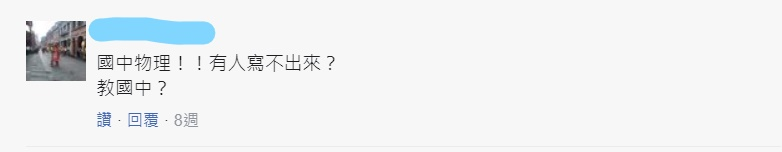
\includegraphics[height=0.2\linewidth]{./resources/physics/sour.jpg}}
\end{itemize}

\subsubsection{核心觀念}
\paragraph{數學}
\begin{itemize}
    \item{純量}
        \SubItem{只有大小、沒有方向、可用實數表示的一個量}
    \item{向量}
        \SubItem{內積}
            \SubSubItem{內積在物理引擎模擬時通常都是用在投影上,代表一條向量到另外一條向量的投影量}
            \SubSubItem{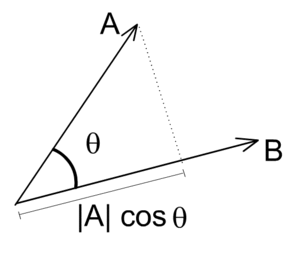
\includegraphics[height=0.2\linewidth]{./resources/physics/intersect.png}}
        \SubItem{外積}
            \SubSubItem{外積通常擔任的身分都是旋轉居多,在三維空間的外積通常表示兩向量維出紙面或入紙面的旋轉,在二維則為順時針旋轉跟順時針旋轉居多}
            \SubSubItem{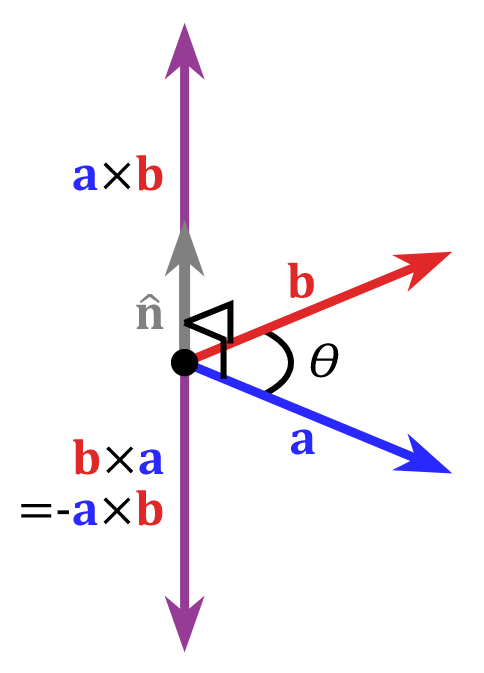
\includegraphics[height=0.2\linewidth]{./resources/physics/outersect.png}}

\item{座標轉換}
        \SubItem{利用線性代數座標空間觀念來方便我們做運算}
        \SubItem{A為旋轉矩陣}
            \SubSubItem{$\begin{bmatrix}x^{'}\\y^{'}\end{bmatrix} = \begin{bmatrix}cos\theta&-sin\theta\\sin\theta&cos\theta\end{bmatrix}\begin{bmatrix}x\\y\end{bmatrix}$}
        \SubItem{$A^{-1} \cdot p$}
            \SubSubItem{將world space轉換到p的local space}
        \SubItem{$A^{1} \cdot p$}
            \SubSubItem{將$p$的`local space`轉換到`world space`}
       \SubItem{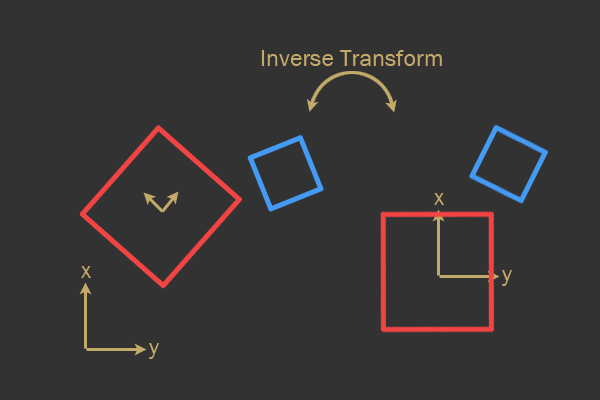
\includegraphics[height=0.5\linewidth]{./resources/physics/inverseTransform.png}}
            \note{左下角為worldSpace的座標,紅框裡的則為各個物體的localspace座標}
\end{itemize}

\paragraph{物理}
\subparagraph{線性相關}

\begin{itemize}
    \item{牛頓力學}
        \SubItem{定律一}
            \SubSubItem{物體在無外力的作用下,會傾向於維持靜止不動,或繼續固定的速度在一直線上運動,這就是慣行的觀念}  
        \SubItem{定律二}
            \SubSubItem{物體的加速度與作用於該物體上的何立成正比,加速度方向與作用力方向相同}  
            \SubSubItem{$F = m \cdot a$}
        \SubItem{定律三}
            \SubSubItem{對於作用於物體上的力,都有一個大小相同案方向相反的反作用力,且作用力與反作用力位在一條線上}  
    \item{物理參數}
        \SubItem{質量m}
        \SubItem{位置x}
        \SubItem{速度v}
            \SubSubItem{$x = v \cdot \Delta t$}
        \SubItem{加速度a}
            \SubSubItem{牛二 - $F = m \cdot a$}
        \SubItem{動量}
            \SubSubItem{向量,意義是物體在其運動方向上保持運動的趨勢}
            \SubSubItem{$P = m \cdot v$}
        \SubItem{衝量}
            \SubSubItem{單位時間內的動量變化量}
            \SubSubItem{$J = \Delta{P} = m \cdot \Delta{v} = F \cdot \Delta{t}$}
\end{itemize}

\subparagraph{角度相關}
\begin{itemize}
    \item{力矩 $\tau$}
        \SubItem{$\tau = F \cdot d$}
        \SubItem{$d$為受力點與質心的距離}
        \SubItem{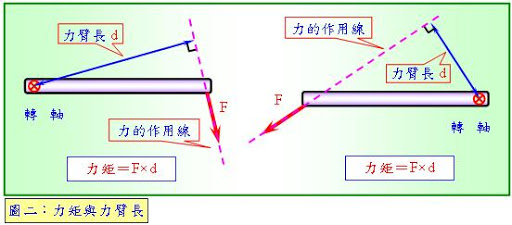
\includegraphics[width=0.5\linewidth]{./resources/physics/tau.png}}
    \item{轉動慣量(慣性矩)$I$}
        \SubItem{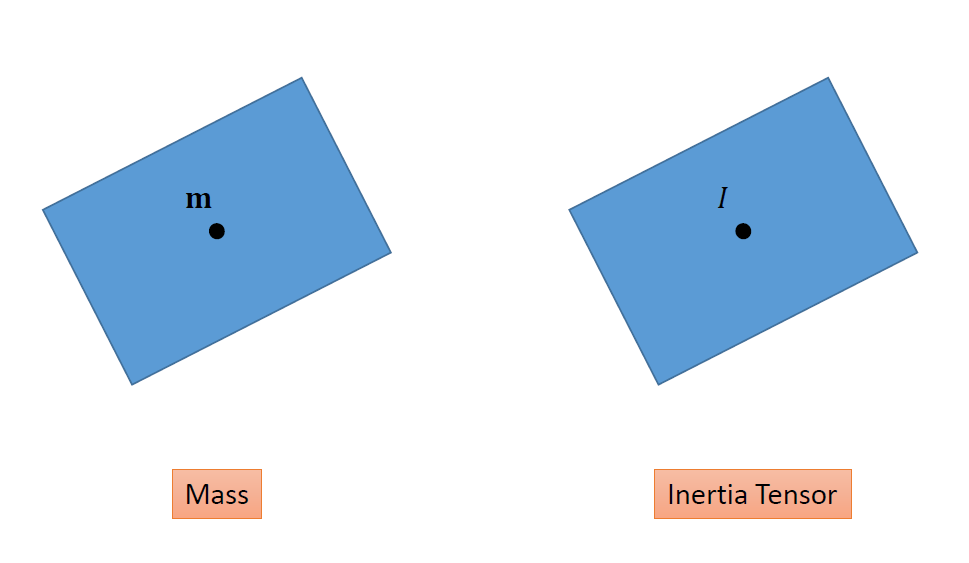
\includegraphics[width=0.5\linewidth]{./resources/physics/Interia.png}}
        \note{既然線性中有質量,在旋轉上也就有所謂的轉動慣量}
        \SubItem{定義}
            \SubSubItem{$I = \sum{m_i r_i^2} = \int_V \rho r^2 dV$}
        \SubItem{拿同樣質量的物體做旋轉時,因參考點的不同,導致有慣性的力量出現}
            \SubSubItem{e.g. 筆拿不同邊,甩的時候力量不一樣,拿邊邊要用比較多力,拿中間甩起來比較輕鬆}
        \SubItem{2D 矩形的質心慣性矩}
            \SubSubItem{質量為 $m$,寬度為 $w$,高度為 $h$ 的二維}
            \SubSubItem{$I = \frac{m(h^2+w^2)}{12}$}
        \SubItem{圓形的質心慣性矩}
            \SubSubItem{質量為M,半徑為r}
        \SubItem{二維的轉動慣量為單一值,三維則是$3*3$的矩陣}
        \note{各種不同的慣性矩如下: https://en.wikipedia.org/wiki/List\_of\_moments\_of\_inertia}
    \item{牛二旋轉版,角加速度$\alpha$}
        \SubItem{線性有 $F = ma$,物體的角加速度($\alpha$)與物體所受的轉矩($\tau$)成正比,其方向跟轉矩的方向相同}
        \SubItem{$\tau = I \alpha$, $\alpha = \frac{\tau}{I}$}
        \SubItem{$\alpha$ 為角加速度}
    \item{角速度}
        \SubItem{算出物體旋轉的角度}
        \SubItem{$\omega = \alpha \cdot \Delta t$}
        \SubItem{$\theta = \omega \cdot \Delta t$}
    \item{角動量}
        \SubItem{物體的角動量是物體的位置向量和動量的叉積,通常寫做$\mathbf{L}$}
        \SubItem{$L = r \times p$}
        \SubItem{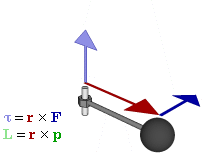
\includegraphics[height=0.2\linewidth]{./resources/physics/L.png}}
\end{itemize}

\subparagraph{微分、積分}
\begin{itemize}
    \item{位置、速度、加速度}
        \SubItem{位置 ---> 速度 ---> 加速度 ($\frac{d}{dt}$) 微分}
        \SubItem{位置 <--- 速度 <--- 加速度 ($\int{dt}$) 積分}
        \SubItem{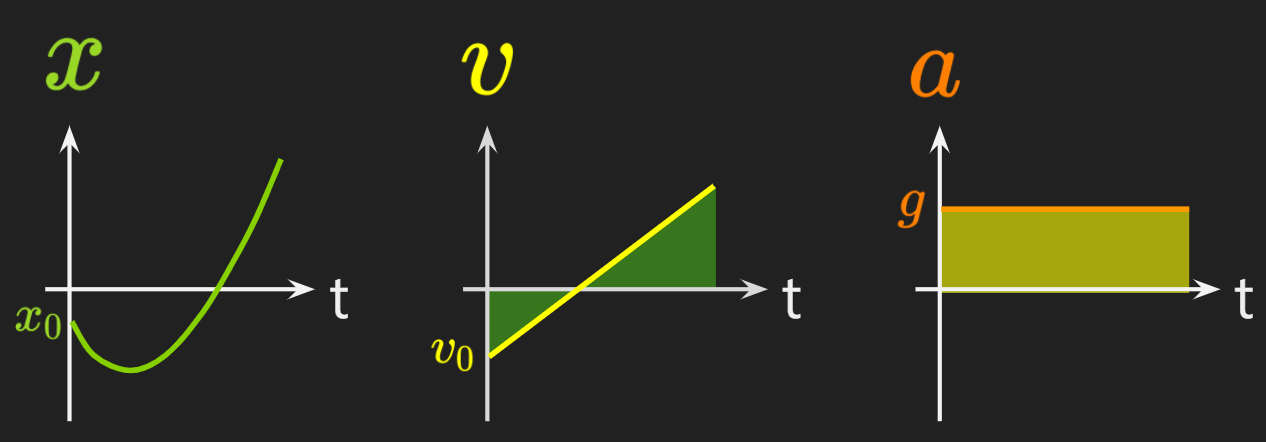
\includegraphics[height=0.2\linewidth]{./resources/physics/xva.png}}
    \item{那,不就找到積分函數就好了?}
        \SubItem{因為我無法知道下一刻的加速度長甚麼樣子,函數圖形有可能會漲跌}
        \SubItem{而只要有力,加速度就會有變化(碰撞、拉扯、浮力(x))}
    \item{因此只能透過數值積分來解決}
        \SubItem{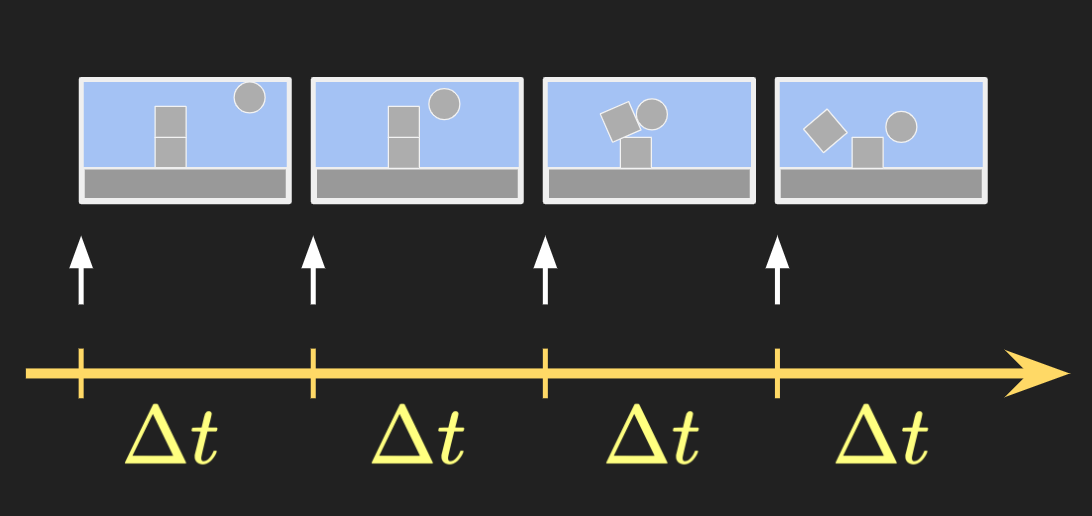
\includegraphics[height=0.2\linewidth]{./resources/physics/deltaT.png}}
    \item{Euler-Method(歐拉法數值積分)}
        \SubItem{用前一刻的值,算出下一刻的值是多少}
            \SubSubItem{程式寫起來可能通常長這樣}
    \begin{lstlisting}
        v += a * dt;
        x += v * dt;
    \end{lstlisting}
    \note{圖片出自: SITCON2020 - 你說這隻溫馴的繩嗎}
    \item{Runge-Kutta \(Runge-Kutta方法\)}
        \SubItem{以 3rd Runge-Kutta 舉例}
    \begin{lstlisting}
        void timeStep(body) 
        {
            auto f = [=](StateStep &step, float2 vel, float t) {
                vel += gravity * t;
                step.velocity = vel;
            };
        
            StateStep F0, F1, F2, F3, F4;
            F0.velocity = float2(0,0);
            f(F1, F0.velocity, 0);
            f(F2, F1.velocity / 2, deltaTime / 2);
            f(F3, F2.velocity / 2, deltaTime / 2);
            f(F4, F3.velocity, deltaTime);
        
            auto v0 = body->vel + body->force * deltaTime / body->mass;
            body->vel =  v0 + (F1.velocity + 2 * F2.velocity + 2 * F3.velocity + F4.velocity) / 6;
            body->pos += body->vel * deltaTime;
        }
    \end{lstlisting}
\end{itemize}

\subsubsection{遊戲物理名詞定義}

\paragraph{Rigid Bodies}
\begin{itemize}
    \item{鋼體,能夠忽略形變的物體}
        \SubItem{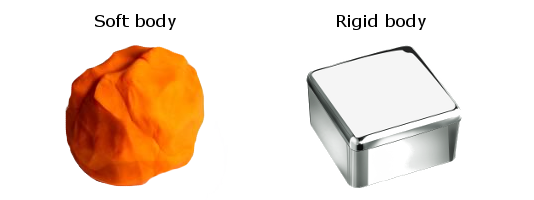
\includegraphics[height=0.2\linewidth]{./resources/physics/rigidBody.png}}
    \note{鋼體與柔體的比較,鋼體例子如鐵盒,柔體例子如黏土}   
\end{itemize}

\paragraph{Joints}
\begin{itemize}
    \item{關節點,能夠連接兩個對象在一個單一的支點}
        \SubItem{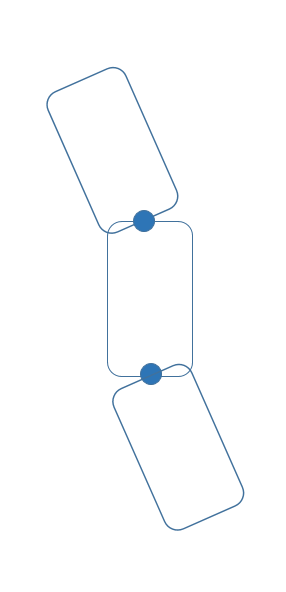
\includegraphics[height=0.2\linewidth]{./resources/physics/Joint.png}}
\end{itemize}

\paragraph{Constraint}
\begin{itemize}
    \item{中文翻譯為約束}
        \SubItem{在遊戲物理的意義,則是讓物體符合遊戲物理世界的規定,像是物體不能穿過地板}
        \SubItem{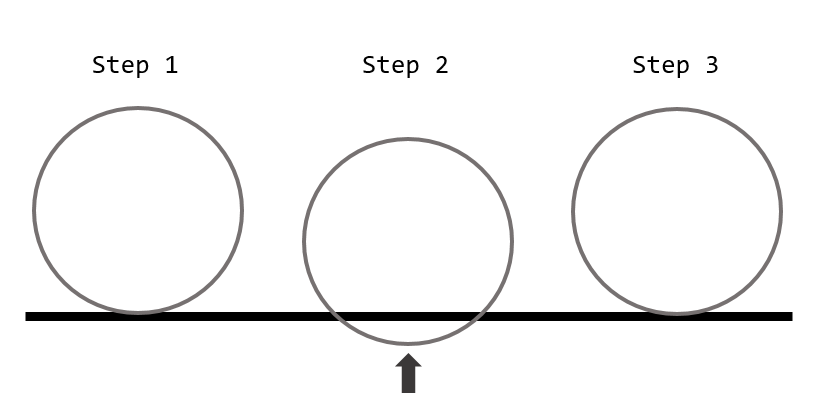
\includegraphics[height=0.2\linewidth]{./resources/physics/Constraint.png}}
\end{itemize}

\paragraph{Contact points}
\begin{itemize}
    \item{在此示意圖中,c1, c2 為接觸點}
        \SubItem{在兩物體重疊之後,會計算出接觸點,透過接觸點來算出如何解掉約束}
        \SubItem{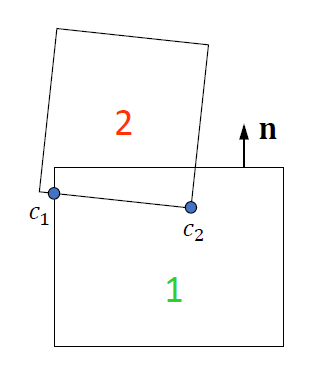
\includegraphics[height=0.2\linewidth]{./resources/physics/contactPoint.png}}
\end{itemize}

\paragraph{Arbiters}
\begin{itemize}
    \item{英文原意,仲裁者}
        \SubItem{每個Aribiter都會有兩個contact-point,以及兩個RigidBody(一個攻、一個受),計算出該point應該要修正的衝量大小}
        \SubItem{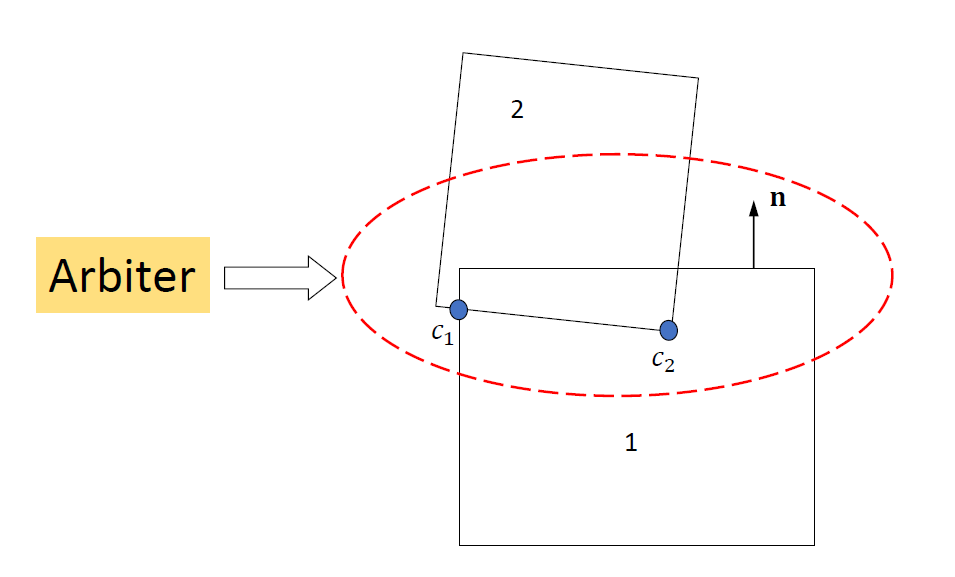
\includegraphics[height=0.2\linewidth]{./resources/physics/Arbiter.png}}
\end{itemize}

\subsubsection{實作}

\paragraph{前言}
\includegraphics[height=0.2\linewidth]{./resources/physics/pre.png}

\begin{itemize}
    \item{依據Box2D作者描述,使用衝量模擬有以下優點}
    \SubItem{Most people don't hate impulses}
        \SubSubItem{大家不討厭衝量}
    \SubItem{The math is almost understandable}
        \SubSubItem{數學總是好懂得}
    \SubItem{Intuition often works}
        \SubSubItem{較直覺去實現}
    \SubItem{Impulses can be robust}
        \SubSubItem{衝量可以較為穩定}
\end{itemize}

\note{內容出自Box2d Lite投影片}   

\paragraph{模擬流程}
% 圖 https://i.imgur.com/DslX81z.png
% figure 遊戲物理模擬示意圖
\paragraph{分析受力 \(Compute Force\)}

\begin{itemize}
    \item{ComputeForce}
        \SubItem{透過受到的力,算出物體的速度及加速度}
        \SubItem{若$mass=0$,則不更新}
        \SubItem{$v$ += $\Delta_{t} * (g + \frac{F}{m} )$ }
        \SubItem{$\omega$ += $\Delta_{t} * \frac{\tau}{I}$}
\end{itemize}

\begin{lstlisting}
if (invMass == 0.0f)
    return;
else
{
    velocity += delta_t * (gravity + invMass * force);
    angularVelocity += delta_t * invI * torque;
}
\end{lstlisting}


\paragraph{更新速度 \(Update Velocity\)}

\begin{itemize}
    \item{Integrate Velocities}
        \SubItem{對速度、速度做積分,能知道position與rotation實際的值}
        \SubItem{$pos$ += $\Delta_{t} * v$}
        \SubItem{$rot$ += $\Delta_{t} * \omega$}
\end{itemize}

\begin{lstlisting}
for (int i = 0; i < (int)bodies.size(); ++i)
{
    Body* b = bodies[i];

    b->position += dt * b->velocity;
    b->rotation += dt * b->angularVelocity;

    b->force.Set(0.0f, 0.0f);
    b->torque = 0.0f;
}
\end{lstlisting}

\paragraph{碰撞檢測、找出接觸點 \(Collision Detection\)}

\subparagraph{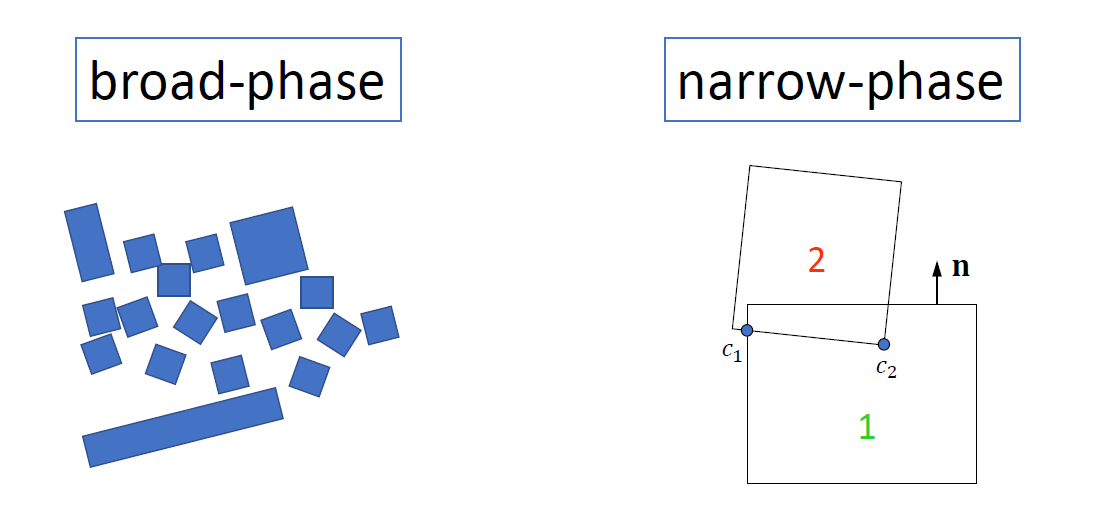
\includegraphics[height=0.4\linewidth]{./resources/physics/detection.png}}

\subparagraph{Broad-phase\(大略檢測\)}

\begin{itemize}
    \item{暴力法\(Brute Force\)}
        \SubItem{運用迴圈偵測每兩兩個物體,並判斷是否有無碰撞}
        \SubItem{Box2D Lite 使用的是 $O(N^2)$ 算法,在實際的Box2D引擎中,採用的是AABB Tree, grid等等的優化演算法,以利於加速整個引擎的碰撞判斷}
    \item{四叉樹\(QuadTree\)}   
        \SubItem{四叉樹(QuadTree)是一種劃分2D區域的樹狀資料結構,類似一般的二元樹,不過子節點為4個}
        \SubItem{可以用來加速碰撞的粗估判斷}
        \SubItem{\href{https://gamedevelopment.tutsplus.com/tutorials/quick-tip-use-quadtrees-to-detect-likely-collisions-in-2d-space--gamedev-374}{QuadTree細節}}
\end{itemize}


\subparagraph{Narrow-Phase (實際檢測) - 碰撞演算法}
\begin{itemize}
    \item{AABB}
    \SubItem{簡介}
        \SubSubItem{為了方邊物體之間進行碰撞檢測運算,通常會對物體創建一個長方形將其包圍,AABB包圍盒也被稱為軸對齊包圍盒}
        \SubSubItem{以矩形包圍物體}
        \SubSubItem{矩形的每條邊,皆與坐標系的軸垂直}
    \SubItem{缺點}
        \SubSubItem{當物體旋轉時就無法檢查}
        \SubSubItem{只能檢查矩形問題}
    \SubItem{實作(需同時滿足兩個條件}
        \SubSubItem{$A.max > B.min$}
        \SubSubItem{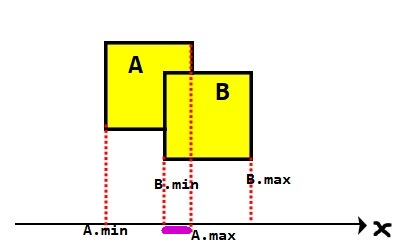
\includegraphics[height=0.4\linewidth]{./resources/physics/AmaxBmin.png}}
        \SubSubItem{$B.max > A.min$}
        \SubSubItem{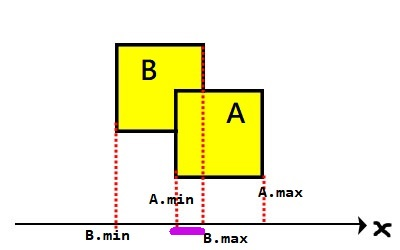
\includegraphics[height=0.4\linewidth]{./resources/physics/BmaxAmin.png}}
    \SubItem{Example Code}
        \begin{lstlisting}
            bool CheckCollision(Shape &a, Shape &b) // AABB - AABB collision
            {
                // x-axis
                bool collisionX = a.Position.x + a.Size.x >= b.Position.x &&
                    b.Position.x + b.Size.x >= a.Position.x;
                // y-axis
                bool collisionY = a.Position.y + a.Size.y >= b.Position.y &&
                    b.Position.y + b.Size.y >= a.Position.y;
                return collisionX && collisionY;
            }  
        \end{lstlisting}
\note{圖片參考自: http://davidhsu666.com/archives/gamecollisiondetection/}
    \item{SAT \(Seperated Axis Therom\)}
        \SubItem{優點}
            \SubSubItem{可以判斷旋轉時的物體之碰撞}
        \SubItem{缺點}
            \SubSubItem{無法檢查凹多邊形,但是能透過將多個凸多邊形組合成凹多邊形的形狀,來作碰撞檢測
SAT必須檢查所有的法向量,來確保物體之間沒有分離線,越多的物體發生碰撞,效率也就越低}
        \SubItem{演算法細節請參考以下連結}
        \note{https://hackmd.io/bo-sYg9TQhyGgpWfJoWC2Q?view}
    \item{GJK \(Gilbert-Johnson-Keerthi\) EPA\(Expanding Polytope Algorithm\)}
        \SubItem{演算法細節請參考以下連結}
        \note{https://hackmd.io/WOPle5lbRzuBzUhgFZ3h5Q}
\end{itemize}

\subparagraph{尋找接觸點和最小穿透軸\(Find Contact Points, Minimum penertration Axis\)}
\begin{itemize}
    \item{在解決約束之前,我們必須要先找到適合的點以及能夠將兩物體分離的向量}
    \item{接觸點}
        \SubItem{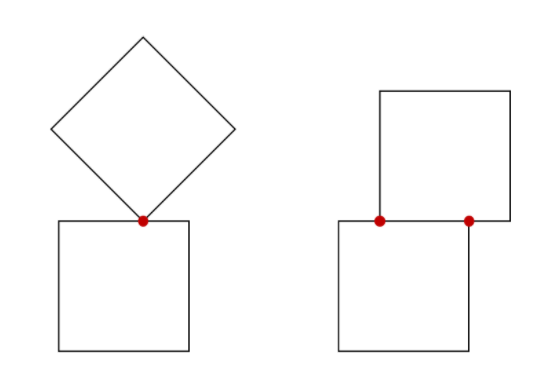
\includegraphics[height=0.4\linewidth]{./resources/physics/contactPoint(2).png}}
        \SubItem{碰撞點是處理碰撞的關鍵,因為這取決了碰撞之後求解器計算出的衝量要應用於物體的哪個位置,在物體的不同位置應用衝量往往會產生截然不同的效果}
            \SubSubItem{舉例,若將接觸點訂在質心,東西則會筆直的向外飛出,而在非質心點的位置,則可能造就物體的旋轉}
    \item{最小穿透軸\(Minimum penertration Axis\)}
        \SubItem{在兩兩物體互相碰撞的狀態下,一定有部分地方邊被插入得比較深,相對的,也會有部分邊被插入得比較淺,或是根本沒有被碰撞到。我們可以透過SAT\(Seperated Axis Therom\)演算法,找出到底哪個地方的邊是被插入最少的,並透過最小穿透軸的法向量,找出最能有效將兩物體分離之向量}
        \SubItem{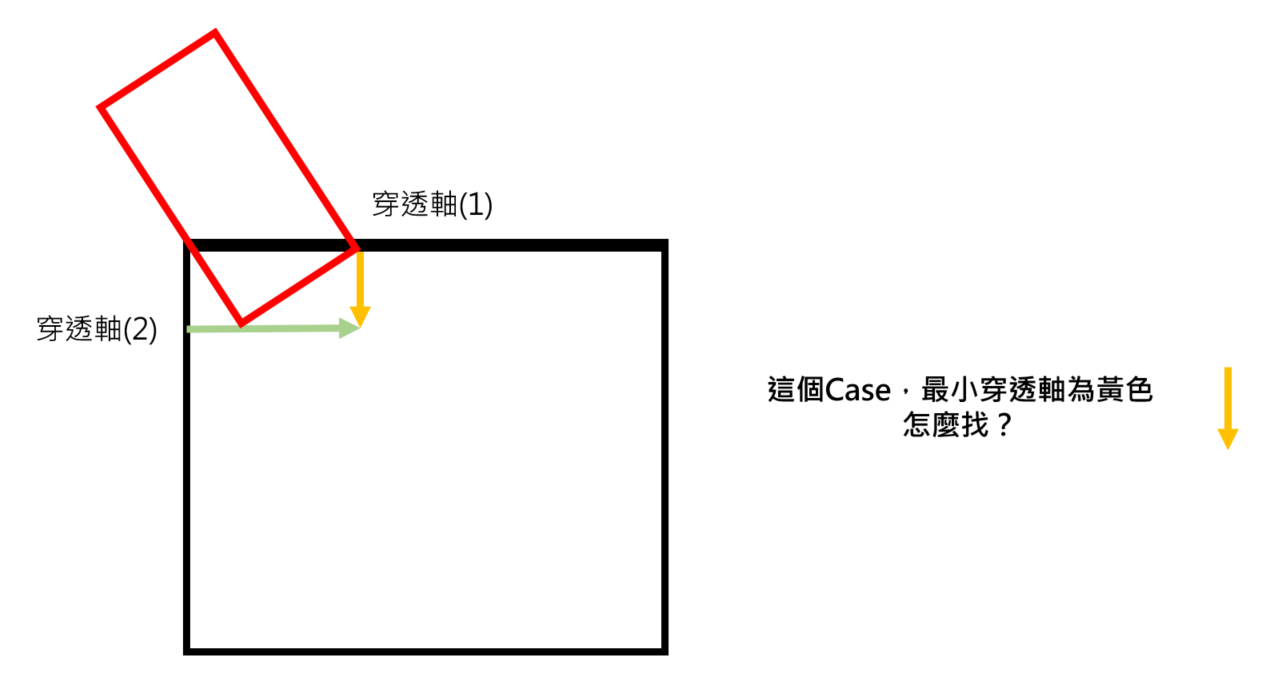
\includegraphics[height=0.4\linewidth]{./resources/physics/miniAxis.png}}
    \item{Reference Face \/ Incident Face}
        \SubItem{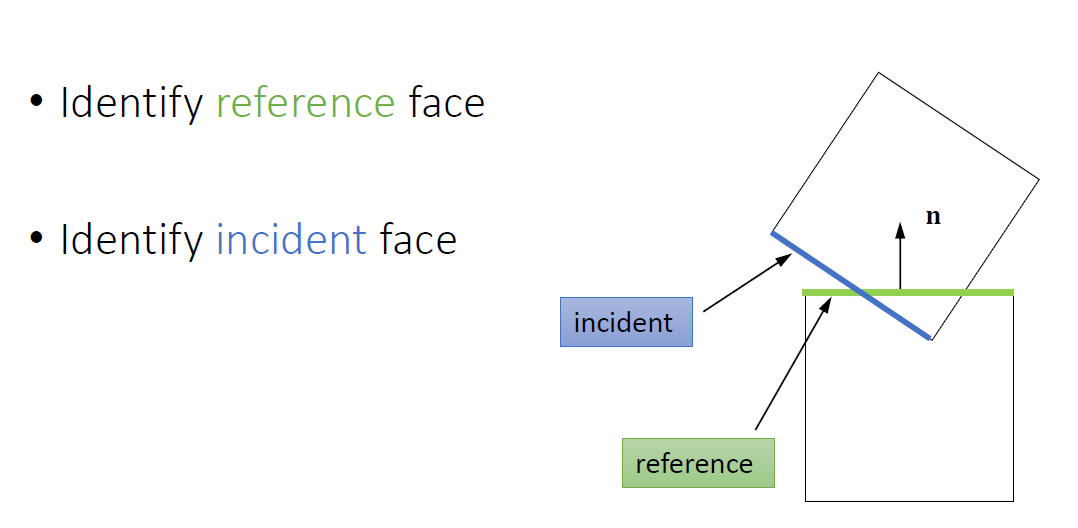
\includegraphics[height=0.4\linewidth]{./resources/physics/refinc.png}}
        \SubItem{找出最小穿透軸之後,我們會決定incident face及reference face,reference代表被插入的邊,incident face則是插入的邊}
    \item{V-Clip演算法}
        \SubItem{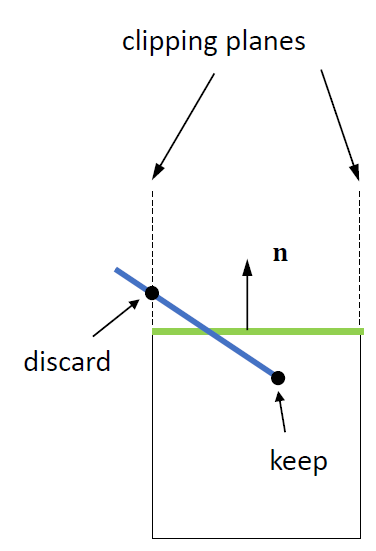
\includegraphics[height=0.4\linewidth]{./resources/physics/vclip.png}}
        \SubItem{透過V-Clip演算法,能夠切除在接觸面以外的接觸點,過濾不必要的接觸點,讓模擬更加穩定及合理,$n$為最小穿透軸的法向量,綠色為reference face,藍色為incident face}
    \item{詳細算法可以參照以下連結}
        \SubItem{https://www.slideshare.net/slideshow/embed\_code/key/5R0vx2057BpeRL} 
\end{itemize}

\paragraph{解決約束 \(Solve Constraints\)}

\begin{itemize}
    \item{約束}
        \SubItem{可以想像成一種在物理世界訂定的規定,遊戲設計者可以依據不同的鋼體物理元素賦予不一樣的規定,讓鋼體有不同的結果。在前一個階段我們計算出接觸點,目的就是藉此用來解決約束}
    \item{約束的例子}
        \SubItem{Contact and Friction}
        \SubItem{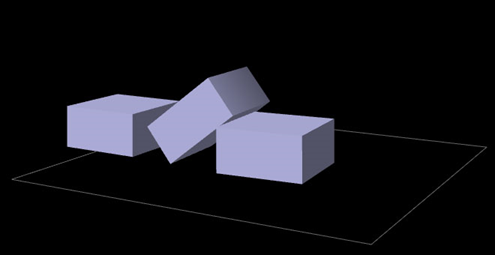
\includegraphics[height=0.4\linewidth]{./resources/physics/contactFric.png}}
        \SubItem{Ragdolls}
        \SubItem{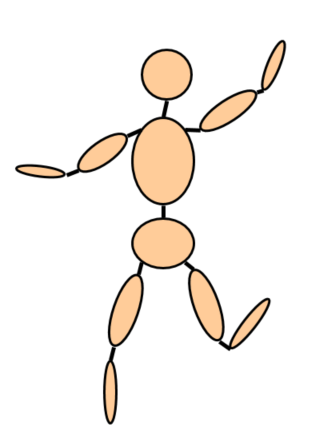
\includegraphics[height=0.4\linewidth]{./resources/physics/Ragdoll.png}}
        \SubItem{Paricles and cloth}
        \SubItem{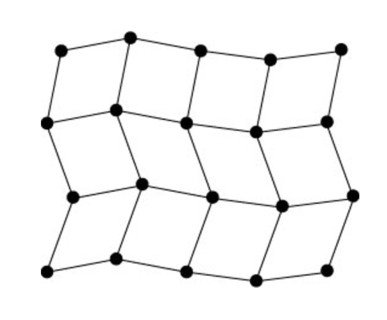
\includegraphics[height=0.4\linewidth]{./resources/physics/PariclesCloth.png}}
\end{itemize}

\note{圖一是接觸與摩擦力約束,圖二是布娃娃的物理系統,詳情可以參考,圖三是用物理粒子連結成一塊布,以上都是約束的例子,圖片出自Erin Catto 2008 Physics PPT}

\subparagraph{位置約束}
\begin{itemize}
    \item{位置約束}
        \SubItem{舉一個簡單的例子,一個人在溜滑板,滑板被限制在坡道上,使人能夠在坡道上安信的划著滑板}
        \SubItem{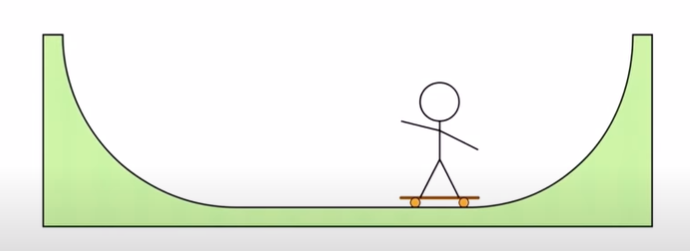
\includegraphics[width=0.4\linewidth]{./resources/physics/position.png}}
        \SubItem{我們可以將滑板當作一個質點,就可以簡單的求出滑板在彎道及平面的約束式子,$C$可以當成一個函數,當$C > 0$,代表滑板在平面或曲面之上,換句話說,一旦我們發現這個函數並不等於0的時候,程式就必須介入來解決約束}
        \SubItem{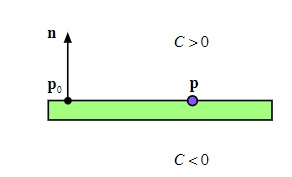
\includegraphics[width=0.4\linewidth]{./resources/physics/plat.png}}
        \note{平面上的約束}
        \SubItem{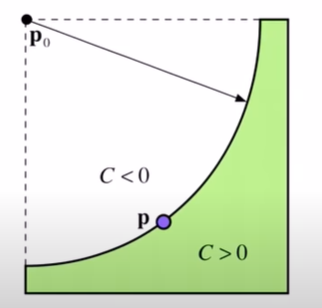
\includegraphics[width=0.4\linewidth]{./resources/physics/curve.png}}
        \note{曲面上的約束}
\end{itemize}

\subparagraph{Ground Constraint\(地面約束\)}
\begin{itemize}
    \item{約束條件,我們不讓物件掉到地下}
        \SubItem{約束條件$y > 0$}
            \SubSubItem{對應的位置約束: $if y <= 0$ 則 $y = 0$}
        \SubItem{對應的速度約束: $V_y = 0$ ?}
            \SubSubItem{若直接對速度直接設定為0,結果會是我碰到地板之後立即停下,但並沒有任何的緩衝}
            \SubSubItem{解決方式:Baumgarte Stabilization}
\end{itemize}

\subparagraph{Baumgarte Stabilization \(邦加特修正\)}

\begin{itemize}
    \item{透過$y$的位置誤差,修正$V_y$}
    \item{$V_y = 0$ -> $V_y + \frac{\beta}{\Delta t} = 0$}
    \item{$\beta$是0~1之間小數}
        \SubItem{beta值越小,不立即修正位置誤差}
        \SubItem{beta值越大,立即修正位置誤差}
        \SubItem{精確的求法,牽涉到更嚴格的磨擦係數}
\end{itemize}

\subparagraph{地面約束實作}

\begin{itemize}
    \item{透過$y$的位置誤差,修正$V_y$}
\end{itemize}

\begin{lstlisting}
float dt = delta_time;
float y = pos.y;
vy += Gravity(重力加速度) * dt;

if (y <= 0.0f)
{
    vy = -(Beta / dt) * y;
}
y += vy * dt;
\end{lstlisting}


\subparagraph{\(Generalization\)通則化}

\begin{itemize}
    \item{我們可以把約束,通則成以下這個矩陣式子}
        \SubItem{$JV + b = 0$}
        \SubItem{$\begin{bmatrix} J_{v1} & J_{v2} \end{bmatrix}\begin{bmatrix} V_{x}\\ V_{y} \end{bmatrix} + b = 0$
            \SubSubItem{J: Jacobian Matrix}
            \SubSubItem{V: Velocity matrix\(速度矩陣\)}
                \SubSubSubItem{線性速度分量}
            \SubSubItem{b: bias\(偏重\)}
                \SubSubSubItem{速度修正項}
    \item{當地面約束套入通則化}
        \SubItem{}$JV + b = 0$}
            \SubSubItem{$V_{y} + \frac{\beta}{\Delta t} = 0$}
            \SubSubItem{$J = \begin{bmatrix}0 & 1\end{bmatrix}$}
                \SubSubSubItem{$x$分量的修正為0,$y$分量的修正係數為1}
            \SubSubItem{$b = \frac{\beta}{\Delta t} y$}
                \SubSubSubItem{偏重修正}
\end{itemize}

\subparagraph{解析速度約束}

\begin{itemize}
    \item{1. $JV + b = 0$}
        \SubItem{此式這就是一個通則,能夠將各個約束套入這個式子,這個過程叫做Generalization}
        \SubItem{J就把他想成修正項,對原先速度的V修正,再加上偏差項}
        \SubItem{在多維度也會適用}
    \item{2️. $M (V_2 - V_1) = L \lambda$}
        \SubItem{$M$ 質量矩陣}
            \SubSubItem{$\begin{bmatrix} M_{1} & 0\\  0 & M_{2} \end{bmatrix}$}
        \SubItem{$V_1$: 一開始違反約束的速度}
        \SubItem{$V_2$: 是修正後的速度}
            \SubSubItem{因此$V_2 - V_1$為速度的修正量}
        \SubItem{$L$: 向量,修正衝量方向}
        \SubItem{$\lambda$: 純量,修正衝量大小}
    \item{我們要算出$L$(修正衝量之方向),$\lambda$(修正衝量之大小) 是多少?}
        \SubItem{3️. $L = J^T$}
            - $J^{T}$為$J$的轉置矩陣
    \item{將3️帶入2️}
        \SubItem{4️$V_2 = V_1 + M^{-1}J^T\lambda$}
    \item{再將4帶入1️,我們知道修正後的速度$V_2$帶入Jacobian的那條式子,一定為0}
        \SubItem{$J(V_1+M^{-1}J^T\lambda)+ b = 0$}
    \item{移項後可得}
        \SubItem{$(JM^{-1}J^T)\lambda = -(JV_1+b)$}
    \item{求得$\lambda$}
        \SubItem{5️ $\lambda = \frac{-(JV_1+b)}{JM^{-1}J^T}$}
    \item{賦予定義}
        \SubItem{$M_{eff}$ 有效質量\(Effective Mass\)}
            - \SubSubItem{6️ $M_{eff} = (JM^{-1}J^T)^{-1}$}
        \SubItem{$\lambda$ 拉格朗日乘數\(Lagrange Multiplier\)}
            - \SubSubItem{7️ $\lambda = M_{eff}*[-(JV_1+b)]$}
\end{itemize}

\subparagraph{距離約束}
\subparagraph{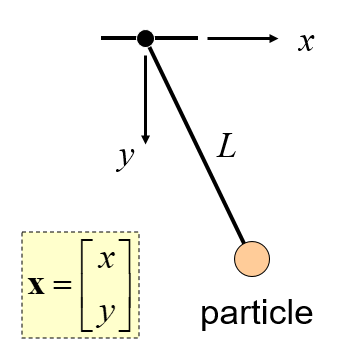
\includegraphics[height=0.4\linewidth]{./resources/physics/disCon.png}}

\begin{itemize}
    \item{他的位置約束的式子長這樣}
        \SubItem{$C = \left \|x  \right \| - L$}
    \item{我們將它進行微分,則能得到速度約束的式子,從此也可以得知,修正衝量的方向為$J^{T}$}
        \begin{equation} C = \left \|x  \right \| - L \end{equation}
        \begin{equation}
            \begin{aligned}
            \frac{dC}{dt}&=&& \frac{d}{dt}\left(\sqrt{x^3+y^2}-L\right) \\
                         &=&& \frac{1}{2\sqrt{x^2+y^2}}\frac{d}{dt}(x^2+y^2)-\frac{dL}{dt}\\
                         &=&& \frac{2(xv_x+yv_y)}{2\sqrt{x^2+y^2}}-0\\
                         &=&& \frac{1}{\sqrt{x^2+y^2}} \begin{bmatrix}x\\y\end{bmatrix}^T \begin{bmatrix}v_x\\v_y\end{bmatrix} \\
                         &=&& \frac{x^T}{\parallel x\parallel}v \\
            \end{aligned}
        \end{equation}
        \begin{equation} \dot{C} = \frac{x^{T}}{\left \|x  \right \|} \cdot v \end{equation}
\end{itemize}

\subparagraph{碰撞回饋}
\subparagraph{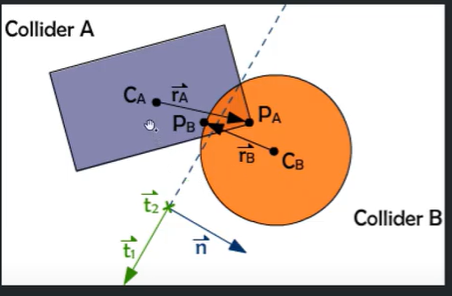
\includegraphics[height=0.5\linewidth]{./resources/physics/feedback.png}}

\begin{itemize}
\item{質心$C_A$, $C_B$}
    \SubItem{穿透點$P_A$, $P_B$}
    \SubItem{向量$\vec{r_A}$, $\vec{r_B}$}
    \SubItem{兩者能夠最有效分開的法向量為$\vec{n}$}
        \SubSubItem{$\vec{n}$的切線向量為$\vec{t1}$, $\vec{t2}$}
\end{itemize}

\begin{itemize}
    \item{需要Constraints的條件}
        \SubItem{位置約束}
            \SubSubItem{$(P_{B}- P_{A}) \cdot n \geq 0$}
                \SubSubSubItem{$P_{A}$指向$P_{B}$的向量投影在$\vec{n}$上}
                \SubSubSubItem{若內積<0,代表碰撞}
            \SubSubItem{$(C_{B} + r_{B} - C_{A} - r_{A}) \cdot \vec{n} \geq 0$}
                \SubSubSubItem{換句話呈現,拆成點與向量}
    \item{速度約束}
        \SubItem{$(-V_{A} - \omega_{A} \times r_{A} + V_{B} + \omega_{B} \times r_{B}) \cdot n \geq 0$}
        \SubItem{這兩點的相對速度在法向量$\vec{n}$上,是要能分開的,也就不會越陷越深}
\end{itemize}

\begin{itemize}
    \item{通則化}
        \begin{equation}
            \begin{aligned}
                \dot{C} &=&& (v_{p2}-v_{p1})\cdot n \\
                        &=&& \begin{bmatrix}v_2+w_2\times(p-x_2)-v_1-w_1\times(p-x_1)\end{bmatrix}\cdots n \\
                        &=&& \underbrace{
                                \begin{bmatrix}
                                    -n \\
                                    -(p-x_1)\times n \\
                                    n \\
                                    (p-x_2)\times n\\
                                \end{bmatrix}^T
                            }_J
                            \begin{bmatrix}
                                v_1 \\
                                w_1 \\
                                v_2 \\
                                w_2 \\
                            \end{bmatrix} \\
            \end{aligned}
        \end{equation}
        \begin{equation}
            A\cdot(B\times C) = C\cdot(A\times B) = B\cdot(A\times C)
        \end{equation}
    \item{通則化結果}
        \begin{equation}
            \begin{aligned}
            JV + b \geq 0 && v = \begin{bmatrix}V_A\\w_A\\V_B\\w_B\end{bmatrix}
            \end{aligned}
        \end{equation}
        \begin{equation}
            J=\begin{bmatrix}-n^T&(-r_A\times n)^T&n^T&(r_B\times n)^T\end{bmatrix}
        \end{equation}
        \begin{equation}    
            \begin{aligned}
                \lambda=\frac{-(JV_1+b)}{(JM^{-1}J^T)} && M=\begin{bmatrix}
                                                                M_A & 0 & 0 & 0 \\
                                                                0 & I_A & 0 & 0 \\
                                                                0 & 0 & M_B & 0 \\
                                                                0 & 0 & 0 & I_B \\
                                                            \end{bmatrix}
            \end{aligned}
        \end{equation}
    \item{位置誤差修正\(bias\)}
        \SubItem{$JV +b = 0$}
        \SubItem{$C: (P_{B} - P_{A}) \cdot n$}
        \SubItem{通式與位置約束合併}
            \SubSubItem{$b = \frac{\beta}{\Delta t} C = \frac{\beta}{\Delta t}(P_{B} - P_{A}) \cdot n$} 
            \SubSubItem{如果只套位置約束修正,頂多讓他們兩個不越陷越深,並不會彈開}
        \SubItem{必須要加上速度約束}
            \SubSubItem{$b = \frac{\beta}{\Delta t}(P_{B} - P_{A}) \cdot n + C_{R}(-V_{A} - \omega_{A} \times r_{A} + V_{B} + \omega_{B} \times R_{B}) \cdot n$ }
            \SubSubItem{$C_{R}$為彈性係數,$C_{R} = 1$ 會變完全彈性碰撞,$C_{R} = 0$ 的話會黏上去}
        \SubItem{有效質量的證明方式,因為細節較為繁雜,而提供連結給閱讀者參考}
            \SubSubItem{http://www.dyn4j.org/2010/09/distance-constraint/comment-page-1/}
    \item{結合$M_{eff}$有效質量(分母)和修正的速度和方向(分子),就能得知修正衝量的結果}
        \SubItem{我們預期設定的}
            $\begin{aligned}v_n = 0 && P_n \geq 0 \end{aligned}$
        \SubItem{求得的結果}
            $P_n = max\left(\frac{-\Delta\overline{v}\cdot n}{k_n},0\right)$
    \item{修正衝量算式}
            \SubItem{$\Delta\overline{v} = \overline{v}_2+\overline{w}_2\times r_2-\overline{v}_1 - \overline{w}_1\times r_1$}
            \SubItem{$k_n = \frac{1}{m_1} + \frac{1}{m_2} + \begin{bmatrix}I^{-1}_{1}(r_1\times n)\times r_1 + I^{-1}{2}(r_2\times n)\times r_2\end{bmatrix}\cdot n$}
    \item{Joint}
        \SubItem{距離約束除了碰撞回饋之外,我們可以將其應用在將兩兩物體相連}
\end{itemize}


\subparagraph{摩擦力}

\begin{itemize}
    \SubItem{消除穿透點PA, PB與切面方向t1的相對速度}
    \SubItem{根據Coulomb理論,摩擦力會箝制在以下式子}
        \SubSubItem{Coulomb's law}
            $|\lambda_t|\leq\mu\lambda_n$
        \SubSubItem{In 2D}
            $-\mu\lambda_n\leq\lambda_t\leq\mu\lambda_n$
    \SubItem{一樣,我們可以將其通則化}
    \SubItem{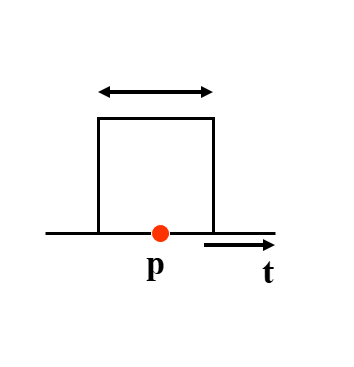
\includegraphics[height=0.4\linewidth]{./resources/physics/pt.png}}
        \begin{equation}
            \begin{aligned}
                \dot{C} &=&& v_p \cdot t \\
                        &=&& \begin{bmatrix}v+w\times(p-x)\end{bmatrix}\cdot t \\
                        &=&& \underbrace{\begin{bmatrix}t\\(p-x)\times t\end{bmatrix}^T}_J \begin{bmatrix}v\\w\end{bmatrix}
            \end{aligned}
        \end{equation}
        \begin{equation}
            \begin{aligned}
                J_n=\begin{bmatrix}-n^T & (-r_A\times n)^T & n^T & (r_B\times n)^T\end{bmatrix}             &&& \lambda_n\geq0 \\
                J_{t_1}=\begin{bmatrix}-t_1^T & (-r_A\times t_1)^T & t_1^T & (r_B\times t_1)^T\end{bmatrix} &&& -\mu\lambda_n\leq\lambda_{t_1}\leq\mu\lambda_n \\
                J_{t_2}=\begin{bmatrix}-t_2^T & (-r_A\times t_2)^T & t_2^T & (r_B\times t_2)^T\end{bmatrix} &&& -\mu\lambda_n\leq\lambda_{t_2}\leq\mu\lambda_n \\
            \end{aligned}
        \end{equation}
    
\end{itemize}

\paragraph{積分結果 \(Integral position\)}

\begin{itemize}
    \SubItem{Example Code}
\end{itemize}

\begin{lstlisting}  
for (int i = 0; i < (int)bodies.size(); ++i)
{
    Body* b = bodies[i];
    b->position += timeStep * b->velocity;
    b->rotation += timeStep * b->angularVelocity;
    b->force.Set(0.0f, 0.0f);
    b->torque = 0.0f;
}
\end{lstlisting}

\paragraph{提升穩定性}

\begin{itemize}
\item{Warm Starting(暖身)}
    \SubItem{為了解決迭代次數過多的問題,我們可以使用暖身(warm starting)的方式來減少迭代次數。在大部分情況下發生碰撞的情況下,每一frame的並不會太大,因此我們可以利用連續的frame來分攤計算的迭代次數。實作非常簡單,在前一幀計算出修正衝量,直接施加在下一個frame上。}
    \SubItem{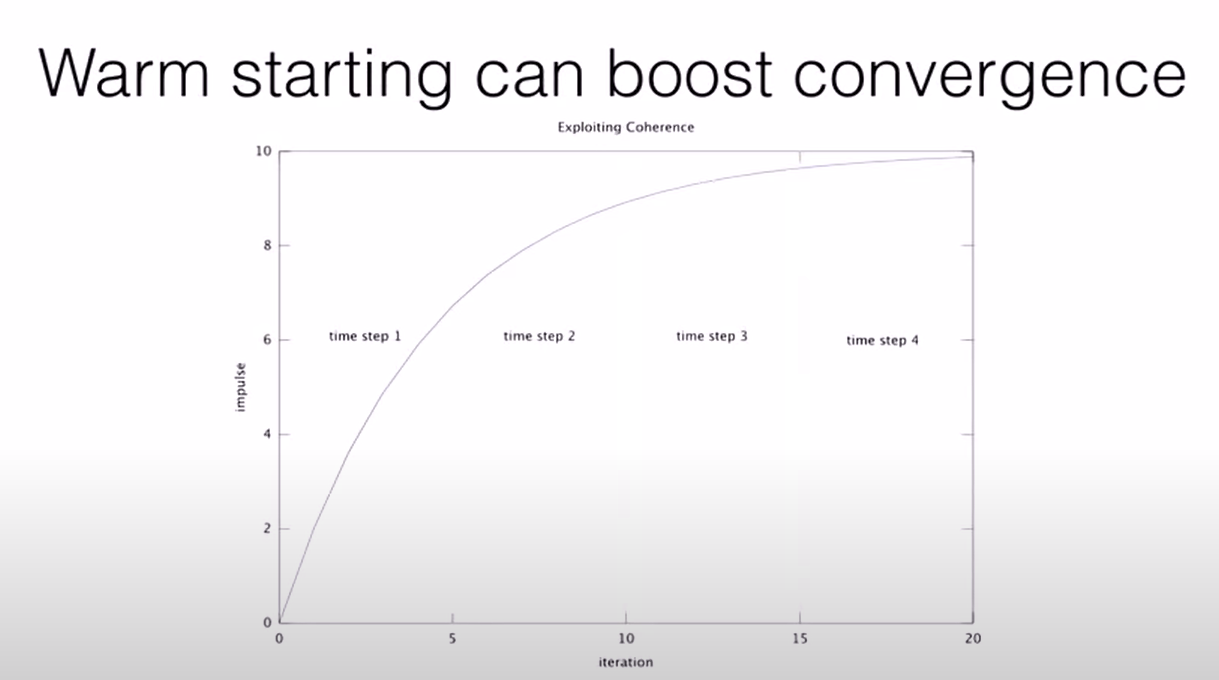
\includegraphics[height=0.4\linewidth]{./resources/physics/warm.png}}
\end{itemize}

\begin{itemize}
    \item{Accumulation Impulse}
        \SubItem{在一般的衝量計算(Box2d稱他為Naïve Impulses)中,每個接觸點算出來的衝量都是獨立出來個別計算的,但這樣會導致微幅的抖動。除此之外,也不能保證每次算出來的修正量值都一定為正,這有可能導致物體會越陷越深的問題}
        \SubItem{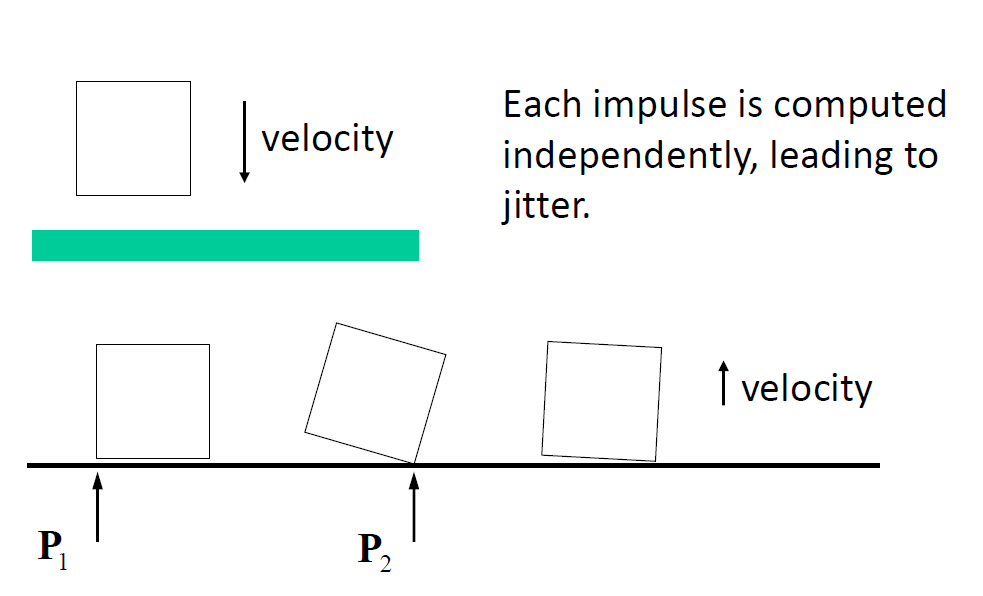
\includegraphics[height=0.4\linewidth]{./resources/physics/accu.png}}
        \SubItem{解決的方法是將每一個frame的衝量都記錄下來,存成一個累積值(accumulation),並將其修正衝量都限制在0以上,就能夠避免越陷越深的問題了,以下使用簡單code來說明}
            \SubSubItem{Normal Clamping}
            \SubSubItem{accmulation\_Pn 累積衝量}
            \SubSubItem{Pn 這一個frame要修正的衝量}
\end{itemize}

\begin{lstlisting} 
temp = accmulation_Pn
accmulation_Pn = max(accmulation_Pn + Pn, 0)
Pn = accmulation_Pn - temp
\caption{}
\end{lstlisting}

\begin{itemize}
    \item{Friction Clamping}
        \SubItem{accmulation\_Pt 摩擦力累積衝量}
        \SubItem{Pt 這一個frame要修正的摩擦力衝量}
        \SubItem{u 為摩擦係數}
\end{itemize}
           
\begin{lstlisting} 
temp = accmulation_Pt
accmulation_Pn = Clamp(accmulation_Pt + Pt, -u*accmulation_Pn, u*accmulation_Pn)
Pt = accmulation_Pt - temp
\end{lstlisting}

\begin{itemize}
    \item{Non \- WarmStarting \& Accumulation}
    \item{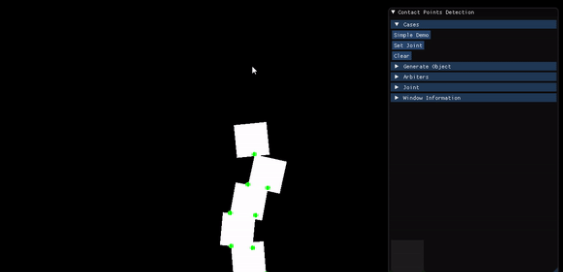
\includegraphics[height=0.4\linewidth]{./resources/physics/none.png}}
    \item{WarmStarting \& Accumulation}
    \item{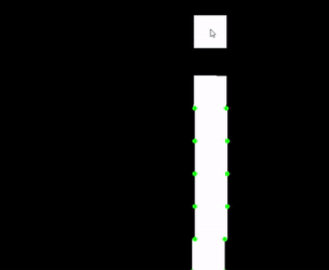
\includegraphics[height=0.4\linewidth]{./resources/physics/has.png}}
\end{itemize}


\paragraph{問題}

\begin{itemize}
    \item{不支援凸多邊形}
        \SubItem{因為使用SAT演算法來找出穿透點,因此無法支援圖多邊形,雖然看到網路上的教學都說把它切成凹多邊形即可,但似乎沒有甚麼東西能夠參考或是資訊可以知道要怎麼切}
    \item{穿隧問題}
        \SubItem{$\Delta t$的不固定,導致每次做數值積分的時候,位置更新都有部分誤差}
\end{itemize}

\paragraph{未來展望}
\begin{itemize}
    \item{新增軟性約束}
        \SubItem{軟性的約束可以模擬彈簧的效果}
    \item{擴展成3D的遊戲物理引擎}
        \SubItem{牽扯到3D,相關運算似乎都要使用一些線性代數中矩陣乘法的一些技巧或是求解器,因為專題時間的關係,無法支援到立體之間的碰撞。}
\end{itemize}
\newpage